\documentclass[]{article}
\usepackage{lmodern}
\usepackage{amssymb,amsmath}
\usepackage{ifxetex,ifluatex}
\usepackage{fixltx2e} % provides \textsubscript
\ifnum 0\ifxetex 1\fi\ifluatex 1\fi=0 % if pdftex
  \usepackage[T1]{fontenc}
  \usepackage[utf8]{inputenc}
\else % if luatex or xelatex
  \ifxetex
    \usepackage{mathspec}
  \else
    \usepackage{fontspec}
  \fi
  \defaultfontfeatures{Ligatures=TeX,Scale=MatchLowercase}
\fi
% use upquote if available, for straight quotes in verbatim environments
\IfFileExists{upquote.sty}{\usepackage{upquote}}{}
% use microtype if available
\IfFileExists{microtype.sty}{%
\usepackage{microtype}
\UseMicrotypeSet[protrusion]{basicmath} % disable protrusion for tt fonts
}{}
\usepackage[margin=1in]{geometry}
\usepackage{hyperref}
\hypersetup{unicode=true,
            pdftitle={Chapter 3 Exercise 3},
            pdfauthor={Allen Church},
            pdfborder={0 0 0},
            breaklinks=true}
\urlstyle{same}  % don't use monospace font for urls
\usepackage{color}
\usepackage{fancyvrb}
\newcommand{\VerbBar}{|}
\newcommand{\VERB}{\Verb[commandchars=\\\{\}]}
\DefineVerbatimEnvironment{Highlighting}{Verbatim}{commandchars=\\\{\}}
% Add ',fontsize=\small' for more characters per line
\usepackage{framed}
\definecolor{shadecolor}{RGB}{248,248,248}
\newenvironment{Shaded}{\begin{snugshade}}{\end{snugshade}}
\newcommand{\KeywordTok}[1]{\textcolor[rgb]{0.13,0.29,0.53}{\textbf{#1}}}
\newcommand{\DataTypeTok}[1]{\textcolor[rgb]{0.13,0.29,0.53}{#1}}
\newcommand{\DecValTok}[1]{\textcolor[rgb]{0.00,0.00,0.81}{#1}}
\newcommand{\BaseNTok}[1]{\textcolor[rgb]{0.00,0.00,0.81}{#1}}
\newcommand{\FloatTok}[1]{\textcolor[rgb]{0.00,0.00,0.81}{#1}}
\newcommand{\ConstantTok}[1]{\textcolor[rgb]{0.00,0.00,0.00}{#1}}
\newcommand{\CharTok}[1]{\textcolor[rgb]{0.31,0.60,0.02}{#1}}
\newcommand{\SpecialCharTok}[1]{\textcolor[rgb]{0.00,0.00,0.00}{#1}}
\newcommand{\StringTok}[1]{\textcolor[rgb]{0.31,0.60,0.02}{#1}}
\newcommand{\VerbatimStringTok}[1]{\textcolor[rgb]{0.31,0.60,0.02}{#1}}
\newcommand{\SpecialStringTok}[1]{\textcolor[rgb]{0.31,0.60,0.02}{#1}}
\newcommand{\ImportTok}[1]{#1}
\newcommand{\CommentTok}[1]{\textcolor[rgb]{0.56,0.35,0.01}{\textit{#1}}}
\newcommand{\DocumentationTok}[1]{\textcolor[rgb]{0.56,0.35,0.01}{\textbf{\textit{#1}}}}
\newcommand{\AnnotationTok}[1]{\textcolor[rgb]{0.56,0.35,0.01}{\textbf{\textit{#1}}}}
\newcommand{\CommentVarTok}[1]{\textcolor[rgb]{0.56,0.35,0.01}{\textbf{\textit{#1}}}}
\newcommand{\OtherTok}[1]{\textcolor[rgb]{0.56,0.35,0.01}{#1}}
\newcommand{\FunctionTok}[1]{\textcolor[rgb]{0.00,0.00,0.00}{#1}}
\newcommand{\VariableTok}[1]{\textcolor[rgb]{0.00,0.00,0.00}{#1}}
\newcommand{\ControlFlowTok}[1]{\textcolor[rgb]{0.13,0.29,0.53}{\textbf{#1}}}
\newcommand{\OperatorTok}[1]{\textcolor[rgb]{0.81,0.36,0.00}{\textbf{#1}}}
\newcommand{\BuiltInTok}[1]{#1}
\newcommand{\ExtensionTok}[1]{#1}
\newcommand{\PreprocessorTok}[1]{\textcolor[rgb]{0.56,0.35,0.01}{\textit{#1}}}
\newcommand{\AttributeTok}[1]{\textcolor[rgb]{0.77,0.63,0.00}{#1}}
\newcommand{\RegionMarkerTok}[1]{#1}
\newcommand{\InformationTok}[1]{\textcolor[rgb]{0.56,0.35,0.01}{\textbf{\textit{#1}}}}
\newcommand{\WarningTok}[1]{\textcolor[rgb]{0.56,0.35,0.01}{\textbf{\textit{#1}}}}
\newcommand{\AlertTok}[1]{\textcolor[rgb]{0.94,0.16,0.16}{#1}}
\newcommand{\ErrorTok}[1]{\textcolor[rgb]{0.64,0.00,0.00}{\textbf{#1}}}
\newcommand{\NormalTok}[1]{#1}
\usepackage{graphicx,grffile}
\makeatletter
\def\maxwidth{\ifdim\Gin@nat@width>\linewidth\linewidth\else\Gin@nat@width\fi}
\def\maxheight{\ifdim\Gin@nat@height>\textheight\textheight\else\Gin@nat@height\fi}
\makeatother
% Scale images if necessary, so that they will not overflow the page
% margins by default, and it is still possible to overwrite the defaults
% using explicit options in \includegraphics[width, height, ...]{}
\setkeys{Gin}{width=\maxwidth,height=\maxheight,keepaspectratio}
\IfFileExists{parskip.sty}{%
\usepackage{parskip}
}{% else
\setlength{\parindent}{0pt}
\setlength{\parskip}{6pt plus 2pt minus 1pt}
}
\setlength{\emergencystretch}{3em}  % prevent overfull lines
\providecommand{\tightlist}{%
  \setlength{\itemsep}{0pt}\setlength{\parskip}{0pt}}
\setcounter{secnumdepth}{0}
% Redefines (sub)paragraphs to behave more like sections
\ifx\paragraph\undefined\else
\let\oldparagraph\paragraph
\renewcommand{\paragraph}[1]{\oldparagraph{#1}\mbox{}}
\fi
\ifx\subparagraph\undefined\else
\let\oldsubparagraph\subparagraph
\renewcommand{\subparagraph}[1]{\oldsubparagraph{#1}\mbox{}}
\fi

%%% Use protect on footnotes to avoid problems with footnotes in titles
\let\rmarkdownfootnote\footnote%
\def\footnote{\protect\rmarkdownfootnote}

%%% Change title format to be more compact
\usepackage{titling}

% Create subtitle command for use in maketitle
\providecommand{\subtitle}[1]{
  \posttitle{
    \begin{center}\large#1\end{center}
    }
}

\setlength{\droptitle}{-2em}

  \title{Chapter 3 Exercise 3}
    \pretitle{\vspace{\droptitle}\centering\huge}
  \posttitle{\par}
    \author{Allen Church}
    \preauthor{\centering\large\emph}
  \postauthor{\par}
      \predate{\centering\large\emph}
  \postdate{\par}
    \date{September 25, 2019}


\begin{document}
\maketitle

Load necessary data and view

\begin{Shaded}
\begin{Highlighting}[]
\KeywordTok{load}\NormalTok{(}\StringTok{"C:/Users/WB537822/Desktop/stats1/Ch3_Exercise3_Height_and_Wages_UK.RData"}\NormalTok{)}

\NormalTok{data <-}\StringTok{ }\NormalTok{dta}

\KeywordTok{View}\NormalTok{(data)}
\end{Highlighting}
\end{Shaded}

3a. Estimate model where height at 33 explains income at age 33. Explain
beta hat 1 and beta hat 0

\begin{Shaded}
\begin{Highlighting}[]
\CommentTok{#Create variables for income and height}
\NormalTok{income <-}\StringTok{ }\NormalTok{data}\OperatorTok{$}\NormalTok{gwage33}
\NormalTok{height <-}\StringTok{ }\NormalTok{data}\OperatorTok{$}\NormalTok{height33}

\CommentTok{#Create OLS model and summarize}
\NormalTok{OLSresults <-}\StringTok{ }\KeywordTok{lm}\NormalTok{(income }\OperatorTok{~}\StringTok{ }\NormalTok{height)}
\KeywordTok{summary}\NormalTok{(OLSresults)}
\end{Highlighting}
\end{Shaded}

\begin{verbatim}
## 
## Call:
## lm(formula = income ~ height)
## 
## Residuals:
##     Min      1Q  Median      3Q     Max 
##  -10.68   -4.96   -3.11   -0.68 2488.68 
## 
## Coefficients:
##             Estimate Std. Error t value Pr(>|t|)
## (Intercept)  -6.5994    12.2143  -0.540    0.589
## height        0.2447     0.1757   1.393    0.164
## 
## Residual standard error: 44.71 on 3694 degrees of freedom
## Multiple R-squared:  0.0005252,  Adjusted R-squared:  0.0002546 
## F-statistic: 1.941 on 1 and 3694 DF,  p-value: 0.1636
\end{verbatim}

The value for beta hat 1 (0.2447) estimates that for each inch in
additional height, the hourly wage increases by 0.2447 pounds. The value
for beta hat 0 (-6.5994) estimates an hourly wage of -6.5994 for someone
with 0 inches of height.

3b. Scatterplot of height and income, identify outliers

\begin{Shaded}
\begin{Highlighting}[]
\KeywordTok{plot}\NormalTok{(height, income, }\DataTypeTok{main=}\StringTok{"Scatterplot of Height and Wage"}\NormalTok{,}
     \DataTypeTok{xlab=}\StringTok{"Height at Age 33 in Inches"}\NormalTok{, }\DataTypeTok{ylab =} \StringTok{"Hourly Wage at Age 33 in Pounds"}\NormalTok{, }\DataTypeTok{pch=}\DecValTok{9}\NormalTok{)}

\KeywordTok{abline}\NormalTok{(}\KeywordTok{lm}\NormalTok{(income }\OperatorTok{~}\StringTok{ }\NormalTok{height, }\DataTypeTok{data=}\NormalTok{data), }\DataTypeTok{col=}\StringTok{'blue'}\NormalTok{)}
\end{Highlighting}
\end{Shaded}

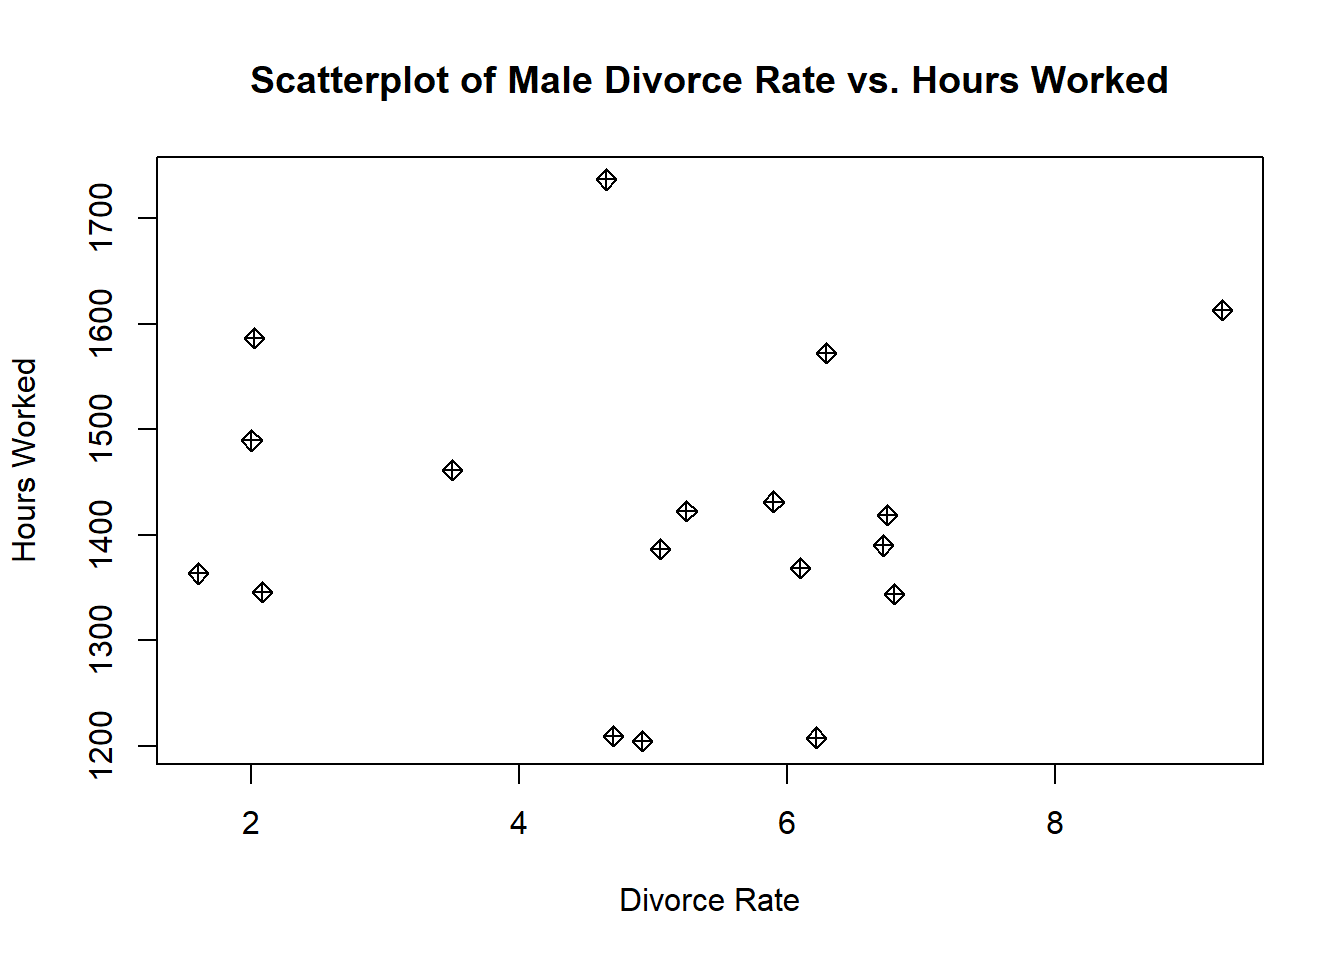
\includegraphics{Ch3set_files/figure-latex/unnamed-chunk-3-1.pdf} The
scatterplot above contains outliers where at least 8 entries have a
height below 30 inches which - while possible - could be outliers.
Additionally, there is an outlier of an individual with a wage of
approximately 2500 pounds per hour.

3c. Create scatterplot, but exclude observations with wages per hour
more than 400 pounds and height less than 40 inches.

\begin{Shaded}
\begin{Highlighting}[]
\CommentTok{#Select rows that match the above specifications}
\NormalTok{newdata <-}\StringTok{ }\KeywordTok{subset}\NormalTok{(data, gwage33 }\OperatorTok{<}\StringTok{ }\DecValTok{400} \OperatorTok{&}\StringTok{ }\NormalTok{height33 }\OperatorTok{>}\StringTok{ }\DecValTok{40}\NormalTok{)}

\KeywordTok{plot}\NormalTok{(newdata}\OperatorTok{$}\NormalTok{height33, newdata}\OperatorTok{$}\NormalTok{gwage33, }\DataTypeTok{main=}\StringTok{"Scatterplot of Height and Wage - Observations Excluded"}\NormalTok{,}
     \DataTypeTok{xlab=}\StringTok{"Height at Age 33 in Inches"}\NormalTok{, }\DataTypeTok{ylab =} \StringTok{"Hourly Wage at Age 33 in Pounds"}\NormalTok{)}

\KeywordTok{abline}\NormalTok{(}\KeywordTok{lm}\NormalTok{(income }\OperatorTok{~}\StringTok{ }\NormalTok{height, }\DataTypeTok{data=}\NormalTok{data), }\DataTypeTok{col=}\StringTok{'blue'}\NormalTok{)}
\end{Highlighting}
\end{Shaded}

\includegraphics{Ch3set_files/figure-latex/unnamed-chunk-4-1.pdf}

The plot above seems to be a more reasonable basis for statistical
analysis because we are now able to see more variance in observations.
It also shows a stronger positive correlation between height and wage.

3d. Reestimate the model from part a but exclude 4 outliers with very
high wages and outliers with height below 40 inches

\begin{Shaded}
\begin{Highlighting}[]
\CommentTok{#Subset newdata and exclude 4 highest wages and height below 40 inches}
\NormalTok{newdata2 <-}\StringTok{ }\KeywordTok{subset}\NormalTok{(newdata, gwage33 }\OperatorTok{<}\StringTok{ }\DecValTok{156} \OperatorTok{&}\StringTok{ }\NormalTok{height33 }\OperatorTok{>}\StringTok{ }\DecValTok{40}\NormalTok{)}

\CommentTok{#Create new OLS model with data that excludes outliers, and summarize results}
\NormalTok{OLSresults2 <-}\StringTok{ }\KeywordTok{lm}\NormalTok{(newdata2}\OperatorTok{$}\NormalTok{gwage33 }\OperatorTok{~}\StringTok{ }\NormalTok{newdata2}\OperatorTok{$}\NormalTok{height33)}
\KeywordTok{summary}\NormalTok{(OLSresults2)}
\end{Highlighting}
\end{Shaded}

\begin{verbatim}
## 
## Call:
## lm(formula = newdata2$gwage33 ~ newdata2$height33)
## 
## Residuals:
##     Min      1Q  Median      3Q     Max 
##  -9.349  -3.698  -1.867   0.498 128.649 
## 
## Coefficients:
##                   Estimate Std. Error t value Pr(>|t|)    
## (Intercept)       -6.95343    4.56052  -1.525 0.127420    
## newdata2$height33  0.23136    0.06543   3.536 0.000411 ***
## ---
## Signif. codes:  0 '***' 0.001 '**' 0.01 '*' 0.05 '.' 0.1 ' ' 1
## 
## Residual standard error: 10.94 on 3663 degrees of freedom
## Multiple R-squared:  0.003402,   Adjusted R-squared:  0.00313 
## F-statistic:  12.5 on 1 and 3663 DF,  p-value: 0.0004112
\end{verbatim}

Having dropped the outliers, the new beta hat 1 is 0.23136 vs.~the old
value of 0.2447. Dropping the outliers weakens the positive correlation
between height and wages. However, an interesting observation is that
standard error for beta hat 1 with outliers removed is 0.06543, whereas
with outliers standard error for beta hat 1 was 0.1757.

3e. What happens when sample size is smaller? Reestimate bivariate ols
model (newdata23), but limit analysis to first 800 observations. Which
changes more from the results with the full sample: the estimated
coefficient on height or estimated standard error of coefficient on
height?

\begin{Shaded}
\begin{Highlighting}[]
\CommentTok{#Create small sample by selecting first 800 rows of the previously subsetted data and verify the number of rows}
\NormalTok{small_sample <-}\StringTok{ }\NormalTok{newdata2[}\DecValTok{1}\OperatorTok{:}\DecValTok{800}\NormalTok{,]}
\KeywordTok{nrow}\NormalTok{(small_sample)}
\end{Highlighting}
\end{Shaded}

\begin{verbatim}
## [1] 800
\end{verbatim}

\begin{Shaded}
\begin{Highlighting}[]
\CommentTok{#Reestimate bivariate ols model with small sample and summarize results}
\NormalTok{OLSresults3<-}\StringTok{ }\KeywordTok{lm}\NormalTok{(small_sample}\OperatorTok{$}\NormalTok{gwage33 }\OperatorTok{~}\StringTok{ }\NormalTok{small_sample}\OperatorTok{$}\NormalTok{height33)}
\KeywordTok{summary}\NormalTok{(OLSresults3)}
\end{Highlighting}
\end{Shaded}

\begin{verbatim}
## 
## Call:
## lm(formula = small_sample$gwage33 ~ small_sample$height33)
## 
## Residuals:
##     Min      1Q  Median      3Q     Max 
##  -8.224  -3.351  -1.616   0.626 111.070 
## 
## Coefficients:
##                       Estimate Std. Error t value Pr(>|t|)  
## (Intercept)            -6.0164     8.0151  -0.751   0.4531  
## small_sample$height33   0.2109     0.1155   1.827   0.0681 .
## ---
## Signif. codes:  0 '***' 0.001 '**' 0.01 '*' 0.05 '.' 0.1 ' ' 1
## 
## Residual standard error: 9.86 on 798 degrees of freedom
## Multiple R-squared:  0.004164,   Adjusted R-squared:  0.002916 
## F-statistic: 3.337 on 1 and 798 DF,  p-value: 0.06811
\end{verbatim}

The re-restimated bivariate OLS model above shows that the estimated
standard error of the coefficient on height changed more when reducing
the original data to 800 observations. Namely, reducing the number of
observations increased the estimated standard error from 0.06543 with
the full set to 0.1155 with the limited set.


\end{document}
